% BeatWeaver draft: current working tree inspected 2026-09-18.
% Confirm author list and affiliation before submission.
\RequirePackage[T1]{fontenc}
\documentclass[conference]{IEEEtran}
\usepackage{cite,balance}
\usepackage{amsmath,amssymb}
\usepackage{graphicx,booktabs,tikz}
\usetikzlibrary{arrows.meta,positioning}
\usepackage[hidelinks]{hyperref}
\newcommand{\vect}[1]{\boldsymbol{#1}}
\newcommand{\R}{\mathbb{R}}
\title{BeatWeaver: Music-Conditioned Humanoid Motion\protect\\
with State-Continuous Smoothing and Transitions}
\author{\IEEEauthorblockN{Chengjun Ouyang}
\IEEEauthorblockA{University College London\\London, United Kingdom}}
\begin{document}
\maketitle
\begin{abstract}
Music-responsive humanoid animation requires both relevant motion selection and
continuous trajectories. Retrieving a suitable dance does not ensure that its
retargeted joint motion is smooth, or that it can be connected to the motion
currently being played. We present BeatWeaver, a causal retrieval-and-synthesis
system for the 29-joint Unitree G1 representation. Streaming audio is compared
with a paired music--motion catalogue using learned music embeddings and
explicit rhythm, tempo, and activity descriptors. Offline, retargeted motions
are regenerated from their human sources and refined by a collision-aware,
receding-horizon quintic planner that preserves accepted position, velocity,
and acceleration. Online, a transition planner searches compatible exit--entry
frame pairs within a musically relevant shortlist and constructs joint-state
bridges subject to continuous polynomial bounds. Boundary-aware time scaling
and modulation connect authored trajectories to these bridges without
predicting future audio. A shared Hermite representation links offline
validation, online planning, and playback. The system produces inspectable
kinematic motion references; physical tracking and comparative performance
remain subjects for evaluation.
\end{abstract}
\begin{IEEEkeywords}
music-driven motion, humanoid animation, motion retrieval, motion retargeting,
trajectory smoothing, transition planning
\end{IEEEkeywords}

\section{Introduction}
Musical rhythm provides timing cues for movement, while timbre, style, and
activity influence its expressive character. These complementary signals make
music an appealing input for interactive humanoid performance. A useful system
must respond to observed audio while maintaining coherent movement as the
music and selected choreography change. For a humanoid representation, this
also requires attention to joint ranges, derivative limits, and geometry.

Music-conditioned dance generation has advanced through paired datasets and
transformer models, learned choreographic codes, and diffusion-based synthesis
\cite{li2021aist,siyao2022bailando,tseng2023edge}. Recent work addresses causal
streaming and direct audio-conditioned humanoid motion
\cite{ji2026discoforcing,li2025freestyle}. These approaches motivate increasingly
responsive interfaces, but generation is not the only useful design choice.
When a finite collection of choreographies is available, retrieval permits
offline inspection and preparation of each motion, explicit selection rules,
and traceable relationships between source data and output.

Retrieval alone leaves two continuity problems unresolved. Within a clip,
retargeting and collision correction can introduce abrupt stops or derivative
changes. Across clips, similar poses can still have incompatible velocities
and accelerations. A blend that interpolates positions does not automatically
preserve the states of the trajectories it joins. Moreover, a trajectory
validated with one interpolation rule may violate constraints when a different
rule is used for playback. These issues motivate treating motion as a sequence
of joint states, rather than a sequence of poses.

We present \emph{BeatWeaver}, a music-conditioned retrieval and kinematic
synthesis system that addresses both continuity problems through a shared
trajectory representation. Music retrieval identifies a relevant motion
neighbourhood. Offline state-aware smoothing prepares its clips; online
state-to-state planning connects them. The transition method is the current
\emph{humanoid matcher v2}, replacing the moving-clip blending method in the
earlier system. Its paired exit--entry search also allows a short terminal
portion of a source clip to be trimmed when an earlier boundary is more
compatible.

The paper describes three contributions:
\begin{itemize}
\item A causal music-to-motion pipeline combining semantic retrieval with
explicit temporal and activity compatibility.
\item An offline, collision-aware smoothing procedure that carries joint
position, velocity, and acceleration through replanning and stores the
same states used by playback.
\item An online transition method combining nonlinear exit--entry scoring,
checked Hermite bridges, and boundary-aware music adaptation.
\end{itemize}
The scope is kinematic reference synthesis. Empirical evaluation is reserved
for Sections~\ref{sec:experiments} and~\ref{sec:results}; physical execution
requires a separate tracking controller.

\begin{figure*}[t]
\centering
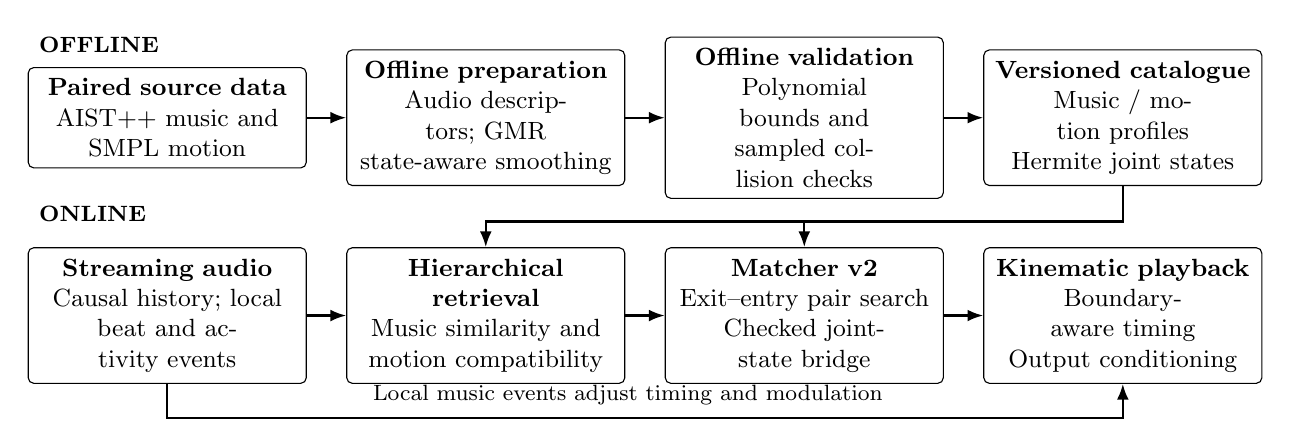
\begin{tikzpicture}[
box/.style={draw,rounded corners=2pt,align=center,text width=3.25cm,
minimum height=1.12cm,font=\small,inner sep=4pt},
flow/.style={-{Latex[length=2mm]},thick},node distance=0.7cm and 0.50cm]
\node[box] (data) {\textbf{Paired source data}\\AIST++ music and\\SMPL motion};
\node[box,right=of data] (offline) {\textbf{Offline preparation}\\Audio descriptors; GMR\\state-aware smoothing};
\node[box,right=of offline] (validation) {\textbf{Offline validation}\\Polynomial bounds and\\sampled collision checks};
\node[box,right=of validation] (library) {\textbf{Versioned catalogue}\\Music / motion profiles\\Hermite joint states};
\draw[flow] (data)--(offline);
\draw[flow] (offline)--(validation);
\draw[flow] (validation)--(library);
\node[box,below=1.00cm of data] (audio) {\textbf{Streaming audio}\\Causal history; local\\beat and activity events};
\node[box,right=of audio] (retrieve) {\textbf{Hierarchical retrieval}\\Music similarity and\\motion compatibility};
\node[box,right=of retrieve] (plan) {\textbf{Matcher v2}\\Exit--entry pair search\\Checked joint-state bridge};
\node[box,right=of plan] (play) {\textbf{Kinematic playback}\\Boundary-aware timing\\Output conditioning};
\draw[flow] (audio)--(retrieve);
\draw[flow] (retrieve)--(plan);
\draw[flow] (plan)--(play);
\draw[flow] (library.south)--++(0,-0.45)-| (plan.north);
\draw[flow] (library.south)--++(0,-0.45)-| (retrieve.north);
\draw[flow] (audio.south)--++(0,-0.43)-| (play.south);
\node[font=\footnotesize,anchor=north] at (5.85,-3.27)
{Local music events adjust timing and modulation};
\node[anchor=west,font=\footnotesize\bfseries] at (-1.75,0.93) {OFFLINE};
\node[anchor=west,font=\footnotesize\bfseries] at (-1.75,-1.22) {ONLINE};
\end{tikzpicture}
\caption{BeatWeaver overview. Both offline smoothing and online transitions
use joint position, velocity, and acceleration. Offline geometric validation
does not certify newly synthesized transitions or physical tracking.}
\label{fig:architecture}
\end{figure*}

\section{Related Work}
\subsection{Music-Conditioned Motion}
AI Choreographer introduces AIST++ and FACT, pairing 3D dance with music and
learning cross-modal temporal relationships \cite{li2021aist}. Bailando
represents dance using a learned choreographic memory and composes motion
units with an actor--critic transformer \cite{siyao2022bailando}. EDGE uses
diffusion for editable music-conditioned dance and incorporates contact-related
physical plausibility considerations \cite{tseng2023edge}. These methods
generate human motion; a humanoid application additionally needs an embodiment
mapping and an execution strategy.

DiscoForcing explicitly addresses causal, bounded-latency audio-driven
character control \cite{ji2026discoforcing}. RoboPerform investigates
expressive humanoid motion driven by music and speech \cite{li2025freestyle}.
BeatWeaver occupies a complementary point in this design space: it selects and
connects existing robot-space references instead of training an online
choreography generator. Its expressive coverage is consequently limited by
the catalogue, while its selection and transition constraints remain explicit.

\subsection{Music Representation and Motion Retrieval}
Music embeddings learned from Discogs metadata capture relationships that
complement engineered acoustic descriptors \cite{alonso2022discogs}.
Signal-processing libraries such as librosa provide tempo, onset, and spectral
features \cite{mcfee2015librosa}. BeatWeaver combines these feature families
because stylistic similarity does not by itself imply a usable motion speed
or matching event density.

Motion graphs assemble captured motion through transitions between compatible
states \cite{kovar2002graphs}. Learned motion matching develops a compact
learned alternative to database-based motion matching
\cite{holden2020matching}. BeatWeaver shares the use of reusable motion data,
but separates musical relevance from instantaneous boundary compatibility.
It retrieves a music-conditioned shortlist and plans joint-state bridges
online rather than constructing a fixed all-pairs motion graph.

\subsection{Retargeting and Constrained Trajectories}
SMPL supplies a common human-motion representation \cite{loper2015smpl}, while
General Motion Retargeting (GMR) maps human motion to humanoid embodiments.
The GMR study shows that reference-motion quality affects downstream tracking
\cite{araujo2025gmr}. BeatWeaver uses GMR as its retargeter and adds its own
state-aware collision correction and motion-file representation. This
postprocessing is distinct from the published GMR method.

Position, velocity, and acceleration are also central to constrained trajectory
generation. Ruckig constructs synchronized trajectories under derivative
constraints for arbitrary target states \cite{berscheid2021ruckig}.
BeatWeaver provides an optional Ruckig backend; its default method uses quintic
Hermite curves with an explicit duration search. The focus here is the
integration of state-preserving clip preparation, musical retrieval, and
online boundary selection, rather than a new general-purpose trajectory solver.

\section{Method}
\subsection{Problem Formulation and System Overview}
Let $\mathcal{A}_{\leq t}$ denote audio observed by wall time $t$. The
catalogue contains music descriptors, motion profiles, and robot trajectories:
\begin{equation}
\mathcal{D}=\{(\vect{x}_i,\vect{m}_i,M_i)\}_{i=1}^{N}.
\end{equation}
Each trajectory has a floating-base pose and joint states
$\vect{s}_{i,k}=(\vect{q}_{i,k},\vect{v}_{i,k},\vect{a}_{i,k})$, where
$\vect{q}_{i,k}\in\R^{29}$ and derivatives are defined in authored time.
The system chooses a motion index, its playback time, and, when needed, a
transition to another motion using only $\mathcal{A}_{\leq t}$ and stored state.

Fig.~\ref{fig:architecture} separates offline preparation from online
execution. Offline, paired AIST++ music and SMPL motion are converted into
audio descriptors and G1 reference trajectories. Online, audio retrieval,
candidate loading, and transition search run outside the foreground playback
path. The foreground consumes completed plans and emits kinematic poses to
MuJoCo \cite{todorov2012mujoco}. The default matcher v2 update rate is 60~Hz;
this is a configuration, not a hard real-time guarantee.



\subsection{Music Descriptors and Hierarchical Retrieval}
Catalogue audio is converted to mono at 16~kHz and analysed in six-second
windows with a two-second hop. Median removal and percentile amplitude
normalization reduce sensitivity to recording gain. The learned backend
produces a 1,280-dimensional Discogs EffNet embedding $\vect{e}$ and 400 style
activations $\vect{g}$. A 24-dimensional rhythm--timbre vector $\vect{r}$
combines tempo, onset and beat statistics, spectral flux, percussive and band
energy ratios, MFCCs, and spectral contrast.

Matcher v2 maintains a causal history of up to 30~s, beginning analysis after
2~s. It requests retrieval at one-second intervals when the worker is free.
Unlike the six-second catalogue segmentation, the query descriptor summarizes
the currently available history; learned patch outputs are averaged. Thus
longer history offers more context but can retain evidence from earlier
musical passages. No future waveform is used, and busy workers do not receive
an accumulating queue of queries.

Embedding and rhythm vectors are standardized using fixed catalogue statistics
and normalized to unit length. Style vectors are unit-normalized without
standardization. For normalized vectors, define
$s_f(q,n)=(1+\bar{\vect{f}}_q^\top\bar{\vect{f}}_n)/2$.
Segment similarity is
\begin{equation}
S_n=0.70s_e(q,n)+0.20s_r(q,n)+0.10s_g(q,n).
\end{equation}
If style vectors are unavailable, the remaining weights are renormalized.
Track evidence is the mean of its three highest segment scores, or all scores
when fewer than three exist. The default style-first policy combines
track-based genre evidence with broad style-label priors and restricts
retrieval to the leading genre, admitting the runner-up when their scores are
close. Weak beat evidence or persistent non-dance style evidence causes
abstention from new music-driven selection.

Motion profiles add source tempo $b_i$, velocity-derived activity, and the
density and regularity of salient poses. These poses are detected as prominent
valleys in whole-body source-motion velocity. For query tempo $b_q$, consider
$\{b_q/b_i,b_q/(2b_i),2b_q/b_i\}$ to accommodate half/double-time ambiguity.
Choose the ratio $r_i$ closest to one in log space within the configured speed
interval, default $[0.55,1.60]$. If no ratio is admissible, exclude the motion.
Tempo compatibility is
\begin{equation}
S_{\mathrm{tempo},i}=\exp\!\left[-\tfrac12(\log r_i/0.28)^2\right].
\end{equation}
Key-pose compatibility compares playback-scaled key-pose density with a
weighted combination of beat and onset rates, together with an interval
regularity term. Activity compatibility is one minus the absolute difference
between normalized audio and motion activity. The final score is
\begin{align}
S_{\mathrm{motion},i}&=0.50S_{\mathrm{tempo},i}
+0.35S_{\mathrm{key},i}+0.15S_{\mathrm{activity},i},\\
S_i&=0.65S_{\mathrm{track},i}+0.35S_{\mathrm{motion},i}.
\end{align}
These are fixed engineering weights, not learned or experimentally optimized
parameters in this draft.

\subsection{State-Preserving Offline Motion Smoothing}
\label{sec:smoothing}
GMR transfers each SMPL sequence to the target humanoid. BeatWeaver's updated
motion preparation, called \emph{GMR v2} within this project, regenerates the
reference from the original human motion. Filtering an older saved trajectory
cannot reconstruct movement already removed by collision-induced holds.
The revised pipeline first constructs a collision-aware positional guide using
joint displacement optimization, range and speed bounds, and linearized
distance constraints. Nonlinear geometry checks restrict unsafe steps.

The guide is not the final playback trajectory. Starting from an accepted
state $\vect{s}_0$, a receding-horizon planner fits a quintic joint curve over
up to 12 source frames. For horizon duration $T$ and normalized time
$u\in[0,1]$, write
\begin{equation}
Q(u)=\sum_{k=0}^{5}\vect{c}_k u^k,\qquad
\vect{z}=[\vect{q}_T^\top,T\vect{v}_T^\top,T^2\vect{a}_T^\top]^\top.
\end{equation}
The initial position, velocity, and acceleration are fixed; coefficients are
affine in the optimized terminal state $\vect{z}$. Future guide states are
tracking objectives rather than hard endpoint constraints. With $Q^{(d)}$
denoting the $d$th derivative with respect to $u$, the implemented objective
has the form
\begin{equation}
\begin{split}
\min_{\vect{z}}\quad
&\sum_{\ell}\sum_{d=0}^{2}\omega_d
\left\|Q^{(d)}(u_\ell)-T^d\hat{\vect{s}}_{\ell}^{(d)}\right\|^2\\
&+\frac{\lambda_j}{5}\sum_{r=0}^{4}
\left\|T^{-3}Q^{(3)}(r/4)\right\|^2,
\end{split}
\label{eq:offline-objective}
\end{equation}
where $\hat{\vect{s}}_{\ell}^{(0,1,2)}$ denotes guide position, velocity, and
acceleration, $\omega=(1,0.1,0.005)$, and $\lambda_j$ sets a soft physical-time
jerk cost. The jerk term is sampled regularization, not a hard jerk bound.

Bernstein control-point bounds constrain position, speed, and acceleration
throughout the curve. Bounds are applied on four equal subintervals to reduce
conservatism. Signed-distance constraints are relinearized during sequential
quadratic optimization, and a short terminal continuation reserves room for
motion beyond the planning horizon. Candidate curves undergo nonlinear
collision sampling and continuous joint-extrema checks before acceptance.

Only one source-frame interval is committed before replanning. Its ending
position, velocity, and acceleration become the next fixed initial state.
Shorter horizons are tried when necessary. If replanning fails, the remaining
previously validated curve may be consumed; an instantaneous zero-velocity
hold is not inserted into the generated trajectory. When no validated
continuation exists, generation fails. At clip initialization only, estimated
derivatives may be reduced if no incoming state was supplied, and the
adjustment is recorded.

The resulting files retain source frame count and timing and store float64
position, velocity, and acceleration arrays. A checksum binds these arrays to
the frame rate. Playback and transition planning reuse the saved states after
joint-name mapping rather than re-estimating derivatives from poses. The
serialized piecewise Hermite curves are checked again for joint bounds and
dense sampled clearance in both configured robot models. This aligns
validation with the interpolation actually used at authored speed. It does
not establish continuous collision avoidance or validate later time warping.

\subsection{Musical Shortlists and Exit--Entry Search}
\label{sec:pair-search}
Matcher v2 retrieves up to 20 motions and retains at most ten alternatives
whose final and music scores lie within 0.05 and 0.08 of the leading motion,
respectively. The active motion is excluded from this normal shortlist.
The shortlist is frozen for preparation, and a successful plan is retained.
This policy avoids replacing an imminent transition with every new ranking;
it does not use the earlier matcher's consecutive-winner and bar-triggered
switching rule.

For each shortlisted motion $j$, eligible entries include every authored
frame with phase $k/(N_j-1)\leq0.2$. Source exits include reachable frames in
the final two authored seconds of the current clip. Invalid joint boundary
states are filtered first. An early exit must still allow the boundary fade
to begin before that exit and before the original terminal fade. Retaining
the original phase denominator while storing a separate stop time prevents
trimming from rescaling the source motion.

Each exit--entry pair is compared using joint pose, joint velocity, binary
foot-contact state, and root features. For a nonnegative discrepancy $d$ with
soft tolerance $\tau$, define
\begin{equation}
P(d;\tau)=r^2+\kappa\max(r-1,0)^2,\qquad r=d/\tau.
\label{eq:penalty}
\end{equation}
We use $\kappa=4$. This penalty is sensitive below the tolerance and grows more strongly above
it; the tolerance is not a hard rejection threshold. Pose and velocity
penalties are averaged across joints, using tolerances of 5\% of joint range
and 10\% of joint speed limit. The contact term uses the number of mismatched
feet with tolerance one. Root height, tilt, linear velocity, and angular
speed discrepancies use tolerances of 0.025~m, 0.075~rad, 0.25~m/s, and
0.5~rad/s, respectively. Their penalties are averaged to form $C_r$.
The total cost is
\begin{equation}
C_{\mathrm{pair}}=\frac{0.45C_q+0.20C_v+0.20C_c+0.10C_r}{0.95}.
\label{eq:pair-cost}
\end{equation}
Acceleration enters bridge feasibility, not this ranking cost. Music determines
the shortlist and resolves ties; it is not an additional geometric penalty.
Further ties prefer later exits, earlier entries, and a deterministic motion
identifier order. Contact agreement is a heuristic, not a contact-force constraint.

Candidate rows are vectorized per exit and merged in sorted order, avoiding a
full exit-by-entry-by-joint tensor. Bridge construction is attempted in this
order until a feasible pair is found. The resulting choice is the first
successful ranked pair encountered within the preparation deadline, rather
than a globally optimal trajectory.

\subsection{Checked State-to-State Bridges}
\label{sec:bridges}
Given an exit state $(\vect{q}_0,\vect{v}_0,\vect{a}_0)$ and an entry state
$(\vect{q}_1,\vect{v}_1,\vect{a}_1)$, a quintic Hermite bridge of duration $T$
satisfies all six endpoint conditions. With derivatives specified in physical
time, its normalized-time coefficients are
\begin{align}
\vect{c}_0&=\vect{q}_0,\quad
\vect{c}_1=T\vect{v}_0,\quad
\vect{c}_2=\tfrac12T^2\vect{a}_0,\nonumber\\
\vect{d}&=\vect{q}_1-\vect{c}_0-\vect{c}_1-\vect{c}_2,\nonumber\\
\vect{h}&=T\vect{v}_1-\vect{c}_1-2\vect{c}_2,\nonumber\\
\vect{g}&=T^2\vect{a}_1-2\vect{c}_2,\nonumber\\
\vect{c}_3&=10\vect{d}-4\vect{h}+\tfrac12\vect{g},\nonumber\\
\vect{c}_4&=-15\vect{d}+7\vect{h}-\vect{g},\nonumber\\
\vect{c}_5&=6\vect{d}-3\vect{h}+\tfrac12\vect{g}.
\label{eq:hermite}
\end{align}
For each joint, the planner checks
\begin{equation}
q_{\min}\leq q(t)\leq q_{\max},\quad
|\dot q(t)|\leq v_{\max},\quad |\ddot q(t)|\leq a_{\max}
\label{eq:limits}
\end{equation}
throughout $[0,T]$. A jerk bound is also checked when explicitly configured;
the default Hermite configuration has no finite jerk limit.

Duration search starts with a displacement-based estimate and coarse
geometric steps. If those fail, a refined grid with spacing no greater than
2\% covers the interval from the minimum duration, default 0.35~s, to 10~s.
Nonzero endpoint derivatives make feasibility nonmonotonic in duration, so
the displacement estimate is not treated as a lower bound. Failure of this
finite search does not prove that every possible duration is infeasible.

Polynomial checks use sampled rejection followed by Bernstein convex-hull
bounds and bounded subdivision. Uncertain cases fall back to evaluating
endpoints and real stationary points in the interval. Sampled tests can reject
a curve but cannot alone authorize it. The optional Ruckig backend instead
constructs a synchronized jerk-limited trajectory and checks its position
extrema; it requires finite jerk limits for every joint.

Preparation checks cancellation and a conservative remaining-playback deadline
between score rows, bridge attempts, and duration trials. Native solver calls
are not preemptible. If no shortlisted transition is found, a checked replay
to frame zero of the current motion is attempted. One expanded-shortlist retry
may then use new candidates and wider musical margins while time remains.
If no plan is ready at the terminal state, playback holds that pose and records
the failure. This terminal hold lies outside the smooth-transition contract;
its onset need not preserve a nonzero terminal velocity.

\subsection{Boundary-Aware Music Adaptation and Playback}
\label{sec:playback}
An authored joint curve is $Q(s)$, where $s$ is clip time. Music-dependent
time scaling changes its physical derivatives:
\begin{equation}
\dot{\vect{q}}=Q'(s)\dot s,\qquad
\ddot{\vect{q}}=Q''(s)\dot s^2+Q'(s)\ddot s.
\label{eq:time-map}
\end{equation}
Thus a bridge planned from authored derivatives cannot simply meet a clip at
an arbitrary music-dependent rate. BeatWeaver fades the rate toward authored
speed and fades pose modulation toward zero near both boundaries.

Let $s_a$ and $s_b$ be the entry and selected exit times and $h$ the boundary
window, default 0.5~s and reduced for short intervals. Define
\begin{align}
H(u)&=10u^3-15u^4+6u^5,\quad u\in[0,1],\\
w(s)&=\min\!\left\{
H\!\left(\operatorname{clip}_{[0,1]}\tfrac{s-s_a}{h}\right),
H\!\left(\operatorname{clip}_{[0,1]}\tfrac{s_b-s}{h}\right)\right\}.
\end{align}
Playback integrates
\begin{equation}
\begin{aligned}
\dot s&=1+w(s)(r_{\mathrm{music}}-1),\\
\vect{q}_{\mathrm{target}}&=Q(s)+w(s)\Delta\vect{q}_{\mathrm{music}}.
\end{aligned}
\label{eq:boundary-playback}
\end{equation}
The beat controller updates the bounded music rate and timing error without
teleporting the sampler to a new phase. Near boundaries, accumulated phase
correction is cleared. Because the window and its first two derivatives
vanish at each join, playback approaches the authored state under regular
bounded music modulation. The bridge then advances in wall time while the
target clip's entry time remains fixed. On completion, the target resumes from
that entry with wall-time overshoot carried forward.

This construction gives matching joint position, velocity, and acceleration
at successful ideal joins before downstream conditioning. Root position and
orientation are aligned and blended separately; they do not inherit the joint
derivative guarantee. Stateful output limits and optional runtime collision
handling can further modify emitted poses, so final-output continuity and
constraint satisfaction require their own measurements.

\subsection{Implementation Scope}
The prototype uses named-joint G1 trajectories, NumPy-based scoring, ONNX audio
inference, and MuJoCo kinematic playback. Retrieval and motion loading support
separate worker processes; pair search uses a background scoring worker.
Generation identifiers reject stale plans, and early-exit plans arriving after
their fade deadline are discarded. Asynchronous execution avoids deliberately
waiting for planning in the playback loop, but does not establish a worst-case
execution-time bound.

The terms \emph{matcher v2} and \emph{GMR v2} refer to independent components.
The corrected dataset must be selected explicitly; choosing matcher v2 alone
does not regenerate or select corrected clips. Motion provenance and saved
state checks prevent stale interpolation revisions from being treated as
validated data. Offline joint-curve bounds concern authored speed. Sampled
self-collision checks do not certify inter-clip bridges, root dynamics,
balance, ground-contact forces, or hardware tracking.

\section{Experiments}
\label{sec:experiments}
\textit{Reserved for the experimental design. Datasets, baselines, metrics,
operating conditions, and evaluation protocol will be added after the
experiments are selected.}
% Deliberately no thesis/v1 or development benchmark results are reused here.

\section{Results and Discussion}
\label{sec:results}
\textit{Reserved for quantitative results, qualitative comparisons,
ablations, and analysis of failure cases. No empirical claims are made in
this section at the draft stage.}

\section{Conclusion}
BeatWeaver combines causal music retrieval with state-aware humanoid motion
synthesis. Its central design choice is to use a consistent joint-state
representation across offline smoothing, transition planning, and playback.
The revised offline pipeline carries accepted derivatives through
collision-aware replanning, while matcher v2 searches musically relevant
exit--entry pairs and joins them with checked trajectories. Boundary-aware
adaptation reconciles music-dependent playback with authored bridge states.
Evaluation of musical relevance, delivered smoothness, transition availability,
and runtime performance remains to be completed. Physical deployment further
requires a dynamically validated tracking controller.

\balance
\bibliographystyle{IEEEtran}
\bibliography{references}
\end{document}
